\documentclass[11pt,a4paper]{article}

\usepackage[margin=2.35cm]{geometry}
\usepackage{fontspec}
\usepackage{amsmath,amssymb,bm,mathtools}
\usepackage{booktabs,longtable,tabularx,array,multirow}
\usepackage{graphicx}
\usepackage[dvipsnames]{xcolor}
\usepackage{tikz}
\usetikzlibrary{arrows.meta,positioning,fit,shapes.geometric}
\usepackage{enumitem}
\usepackage{microtype}
\usepackage{caption}
\usepackage{natbib}
\usepackage{hyperref}
\usepackage[nameinlink,noabbrev]{cleveref}

\definecolor{deepblue}{HTML}{1F4E79}
\definecolor{softblue}{HTML}{EAF2F8}
\definecolor{deeporange}{HTML}{B45F06}
\definecolor{softorange}{HTML}{FCE5CD}
\definecolor{deepgreen}{HTML}{38761D}
\definecolor{softgreen}{HTML}{D9EAD3}
\definecolor{deepred}{HTML}{990000}
\definecolor{softgray}{HTML}{F3F4F6}

\hypersetup{
  colorlinks=true,
  linkcolor=deepblue,
  citecolor=deepgreen,
  urlcolor=deeporange,
  pdftitle={Toward a Next-Generation First-Principles Theory of Electron--Phonon Coupling},
  pdfauthor={AITP Research Notes}
}

\setlist[itemize]{leftmargin=1.6em,itemsep=0.3em,topsep=0.4em}
\setlist[enumerate]{leftmargin=1.8em,itemsep=0.3em,topsep=0.4em}
\setlength{\parindent}{0pt}
\setlength{\parskip}{0.55em}
\renewcommand{\arraystretch}{1.18}

\newcommand{\dfpt}{\mathrm{DFPT}}
\newcommand{\ks}{\mathrm{KS}}
\newcommand{\mb}{\mathrm{MB}}
\newcommand{\ii}{\mathrm{i}}
\newcommand{\ee}{\mathrm{e}}
\newcommand{\vq}{\bm{q}}
\newcommand{\vk}{\bm{k}}
\newcommand{\vr}{\bm{r}}
\newcommand{\Tr}{\operatorname{Tr}}
\newcommand{\order}{\mathcal{O}}
\newcommand{\claimstatus}[1]{\textsc{#1}}

\newenvironment{keypoint}[1][Key point]
{\vspace{0.35em}\noindent\color{deepblue}\rule{\linewidth}{0.7pt}\par
 \noindent\textbf{#1.}\ \color{black}}
{\par\noindent\color{deepblue}\rule{\linewidth}{0.7pt}\color{black}\vspace{0.35em}}

\title{\textbf{Toward a Next-Generation First-Principles Theory\\of Electron--Phonon Coupling}\\[0.45em]
\large Why DFPT Works, Where It Fails, and a Channel-Resolved Correction Strategy}
\author{AITP Research Notes}
\date{30 July 2026}

\begin{document}

\maketitle

\begin{abstract}
Density-functional perturbation theory (DFPT) is the standard first-principles
method for lattice dynamics and electron--phonon coupling.  Its practical success
extends from simple metals and semiconductors to several materials with appreciable
electronic correlations, even though the physical scattering amplitude is a
many-body vertex and DFPT uses a static Kohn--Sham response.  The central question
of this proposal is therefore not whether corrections to DFPT exist, but why they
are often small for some phonons and large for others.

We formulate a testable working hypothesis: the DFPT error is controlled primarily
by the operator channel in which a phonon perturbs the low-energy electronic
Hamiltonian, together with the channel-resolved many-body susceptibility and its
frequency dependence.  A common charge-like perturbation is constrained in the
strict uniform limit and has a particularly simple realization in the uniform
electron gas.  Orbital splitting, hybridization, hopping, spin, and interaction
modulation are not protected by the same constraint.  This distinction explains
why strong correlation alone is not a sufficient failure criterion and motivates
a next-generation method: preserve DFPT as a low-cost baseline, project each
phonon perturbation into physically defined channels, and add only the static or
dynamic many-body corrections required by those channels.  The proposal specifies
the equations, limits, benchmark materials, falsification criteria, a two-day
literature sprint, and an AI-agent workflow for turning the hypothesis into a
transparent prediction framework.
\end{abstract}

\begin{keypoint}[Proposed deliverable]
The intended result is not a universal scalar multiplier for every
electron--phonon matrix element.  It is a channel-resolved, uncertainty-aware
correction layer on top of DFPT that can also decide when uncorrected DFPT is
already adequate.
\end{keypoint}

\tableofcontents
\listoffigures
\listoftables
\clearpage

\section{Problem statement and scope}
\label{sec:motivation}

In crystalline solids, the interaction between electrons and lattice vibrations
controls electrical resistance, conventional superconductivity, thermoelectric
transport, carrier relaxation, and device heating.  DFPT is the most widely used
first-principles tool for calculating phonons and electron--phonon matrix elements
because it avoids a separate large-supercell calculation for every displacement
and treats the self-consistent electronic response directly
\citep{Baroni2001,Gonze1995,Giustino2017}.

The motivating observation of Quantum Harness Issue 35 is that DFPT is often
quantitatively useful in a surprisingly broad range of materials
\citep{Issue35}.  This statement needs careful wording.  It does \emph{not} mean
that ordinary semilocal DFPT is uniformly accurate for every correlated material,
every phonon, and every observable.  Standard DFPT can fail when the reference
electronic structure is qualitatively wrong, when a phonon couples to an
unprotected internal degree of freedom, or when the electronic response is
strongly frequency dependent.  The real puzzle is narrower and more useful:

\begin{keypoint}[Core scientific question]
Why are corrections beyond static Kohn--Sham linear response small for some
electron--phonon perturbations, including some perturbations in correlated
materials, while they are large for other modes in the same material?
\end{keypoint}

This formulation rules out two incomplete answers.

\begin{enumerate}
  \item \textbf{``The quasiparticle residue cancels the vertex.''}  A numerical
  product close to one is evidence, not a physical explanation.  The Ward identity
  produces such a cancellation only in a specific conserved-charge limit, whose
  order of limits is not the generic adiabatic phonon limit.
  \item \textbf{``DFPT works because the phonon shifts every electronic state by
  the same amount.''}  Real perturbations do not act equally on all Bloch states.
  Even a local operator proportional to the identity inside a correlated orbital
  subspace produces band- and momentum-dependent matrix elements because Bloch
  states have different orbital weights and phases.
\end{enumerate}

The proposal instead treats the one-body derivative of the electronic Hamiltonian
as an operator.  It separates the single global identity
\texttt{global\_charge}, relative block-identity shifts
\texttt{site\_charge}, block-internal traceless structure
\texttt{internal}, and inter-block matrix elements \texttt{nonlocal}.
Derivatives of interaction parameters are two-body vertices in a different
operator space.  Conservation laws can constrain only the first one-body
direction, and only when the original unprojected perturbation is independently
verified as a strict uniform $\vq=0$ full-space common shift.

\subsection{Target deliverable}

The target is a computational framework that uses DFPT as a baseline and adds a
small number of physically interpretable, channel-resolved many-body corrections.
It should be:

\begin{itemize}
  \item \textbf{simpler} than a full many-body calculation of every
  $g_{mn\nu}(\vk,\vq)$;
  \item \textbf{potentially cheaper than a dense beyond-DFPT vertex grid} by
  focusing expensive calculations on risky modes and low-dimensional operator
  channels, without claiming a measured speedup over DFPT;
  \item \textbf{transparent} because every correction is attached to a named
  physical operator and a documented validity test;
  \item \textbf{falsifiable} on materials for which DFPT succeeds for one mode
  but fails for another; and
  \item \textbf{uncertainty-aware}, including an abstention path when a mode lies
  outside the validated regime.
\end{itemize}

The first validation object may be the uniform electron gas (UEG), but it is not
the final theory.  The UEG contains only a scalar density channel and therefore
provides a clean baseline for understanding what is special about that channel.
The proposed method must then survive multi-orbital and correlated-material tests.

\subsection{What is and is not being corrected}

DFPT computes several related quantities: force constants, phonon eigenvectors,
Born effective charges, dielectric response, and electron--phonon matrix elements.
The main target here is the last quantity: the physical quasiparticle scattering
vertex associated with a phonon.  Corrections to equilibrium structure,
anharmonicity, or the phonon spectrum may also matter, but they are separate axes
of error.  The proposed benchmark will keep the following gates distinct:

\begin{enumerate}
  \item the Kohn--Sham ground-state and phonon baseline;
  \item the electron--phonon matrix element $g$;
  \item the observable assembled from $g$, such as a linewidth, mobility, or
  pairing kernel.
\end{enumerate}

Passing one gate does not establish the next.

\section{What standard DFPT actually assumes}
\label{sec:dfpt}

\subsection{The perturbation and the matrix element}

Let $u_{\nu\vq}$ be the normal coordinate of phonon branch $\nu$ and wavevector
$\vq$.  After including the conventional phonon normalization factor, define the
self-consistent Kohn--Sham perturbation operator
\begin{equation}
  D^{\ks}_{\nu\vq}
  \equiv \partial_{\nu\vq} V_{\ks}
  = \partial_{\nu\vq} V_{\mathrm{ion}}
  + \partial_{\nu\vq} V_{\mathrm{Hxc}} .
  \label{eq:dks}
\end{equation}
The DFPT electron--phonon matrix element is
\begin{equation}
  g^{\dfpt}_{mn\nu}(\vk,\vq)
  = \langle \psi_{m,\vk+\vq} |
    D^{\ks}_{\nu\vq}
    | \psi_{n,\vk} \rangle .
  \label{eq:gdfpt}
\end{equation}
The perturbation is a matrix in band, orbital, spin, and reciprocal-lattice
indices.  Therefore standard DFPT does not assume that every electron sees the
same scalar shift.

The first-order orbital response is obtained from a Sternheimer equation of the
schematic form
\begin{equation}
  \bigl(\hat H_{\ks}-\varepsilon_{n\vk}\bigr)
  |\partial_{\nu\vq}\psi_{n\vk}\rangle
  = -\hat Q_{\vk+\vq}
  \bigl(\partial_{\nu\vq}V_{\ks}
  -\partial_{\nu\vq}\varepsilon_{n\vk}\bigr)
  |\psi_{n\vk}\rangle,
  \label{eq:sternheimer}
\end{equation}
where $\hat Q$ projects outside the occupied state or selected variational
subspace.  The induced density updates $V_{\mathrm{Hxc}}$ until self-consistency.

\subsection{Static electronic equilibrium}

In ordinary adiabatic DFPT, the electrons are assumed to remain in the
instantaneous ground state associated with a slowly displaced lattice
\citep{Gonze1995,Baroni2001}.  Equivalently, the electronic response entering
\cref{eq:sternheimer} is evaluated at zero external frequency.  The electronic
denominator contains Kohn--Sham energy differences, but not a phonon-frequency
shift such as $\varepsilon_{m,\vk+\vq}-\varepsilon_{n\vk}\pm\omega_{\nu\vq}$.

This assumption is usually sensible when electronic relaxation and interband
energy scales are fast compared with the phonon period.  It can fail for low
carrier densities, narrow bands, small Fermi energies, polar optical modes,
collective modes, or any situation in which $\omega_{\nu\vq}$ is not negligible
on the scale governing the electronic response.

\subsection{The response equation behind DFPT screening}

For a scalar density perturbation, suppressing matrix indices for clarity,
\begin{align}
  \delta V_{\ks}
  &= \delta V_{\mathrm{ion}}+(v+f_{\mathrm{xc}})\delta n,
  \label{eq:vksresponse}\\
  \delta n &= \chi_s\,\delta V_{\ks},
  \label{eq:chisresponse}
\end{align}
where $v$ is the Coulomb interaction, $f_{\mathrm{xc}}$ is the static
exchange--correlation kernel, and $\chi_s$ is the independent Kohn--Sham density
response.  Solving the two equations gives
\begin{equation}
  \delta V_{\ks}
  = \bigl[1-(v+f_{\mathrm{xc}})\chi_s\bigr]^{-1}
    \delta V_{\mathrm{ion}},
  \qquad
  g^{\dfpt}
  = \frac{g^0}{1-(v+f_{\mathrm{xc}})\chi_s}
  \label{eq:gdfptscalar}
\end{equation}
in a translationally invariant scalar problem.  In a crystal these quantities are
matrices in reciprocal lattice vectors and may also carry spin or sublattice
indices.

\subsection{The precise missing term}

Choose the convention
\begin{equation}
  G^{-1}(\omega)=
  \omega+\mu-H_{\ks}-\Sigma^{\mathrm{corr}}(\omega),
  \label{eq:gconvention}
\end{equation}
where $\Sigma^{\mathrm{corr}}$ is the self-energy correction beyond the chosen
Kohn--Sham reference, with the corresponding double counting removed.  The
many-body perturbation of the quasiparticle equation contains
\begin{equation}
  D^{\mb}_{\nu\vq}(\omega)
  = \partial_{\nu\vq}
    \bigl[V_{\ks}+\Sigma^{\mathrm{corr}}(\omega)\bigr].
  \label{eq:dmb}
\end{equation}
Thus the central vertex term absent from standard DFPT is
$\partial_{\nu\vq}\Sigma^{\mathrm{corr}}$, together with its frequency
dependence and consistent wavefunction renormalization.  A large equilibrium
self-energy does not logically imply a large derivative with respect to a
particular phonon.  This distinction is the first reason why the label ``strongly
correlated'' alone cannot predict the DFPT error.  A consistent separation between
the DFT starting point and many-body electron--phonon corrections is discussed in
detail by \citet{Marini2015}.

\begin{keypoint}[Operational limitation of DFPT]
Standard DFPT is a static Kohn--Sham response.  Its reliability for a physical
quasiparticle vertex depends on whether the phonon derivative of the beyond-DFT
self-energy is small, already represented by the chosen static density
functional, or cancelled by a constraint in the relevant operator channel.
\end{keypoint}

\section{Many-body response, screening, and conservation laws}
\label{sec:manybody}

\subsection{Why screening, polarization, and the vertex are not independent}

In Hedin's closed set of equations, the irreducible polarization $P$, dielectric
function $\epsilon$, screened interaction $W$, and reducible density response
$\chi$ satisfy schematically \citep{Hedin1965,Giustino2017}
\begin{align}
  P &= -\ii GG\Gamma_\rho, \\
  \epsilon &= 1-vP, \\
  W &= \epsilon^{-1}v, \\
  \chi &= P(1-vP)^{-1}.
  \label{eq:hedinresponse}
\end{align}
Here $\Gamma_\rho=-\delta G^{-1}/\delta V_{\mathrm{tot}}$ is a proper density
vertex in the stated convention.  Matrix products and integrations over internal
variables are implicit.  These relations answer an important conceptual question:
screening, the quasiparticle vertex, and static density response are not three
independent physical factors available for arbitrary multiplication.  The vertex
enters $P$; $P$ determines $\epsilon$; and $\chi$ follows from both.  Mixing proper
and screened vertex conventions can therefore count screening twice.

In a scalar electron gas, a convenient schematic form for the quasiparticle
coupling to an external ionic perturbation is
\begin{equation}
  g^{\mathrm{phys}}(\vq,\omega)
  = g^0(\vq)\,
    \frac{z\,\Gamma_\rho(\vq,\omega)}
         {\epsilon(\vq,\omega)},
  \label{eq:gphysical}
\end{equation}
where $z$ is the quasiparticle residue.  This equation is useful only after the
vertex convention and screening factor have been stated.  In this scalar
expression $z\Gamma_\rho$ includes the quasiparticle external-leg residue
appropriate to that convention.  It must not be identified without conversion
with the fixed-basis inverse-Green-function vertex of \cref{eq:dmb}.

\subsection{The Ward identity and its two limits}

Charge conservation and gauge invariance imply the Ward--Takahashi identity
\citep{Nambu1960}
\begin{equation}
  \ii\nu\,\Gamma^0(k+q,k)
  -\vq\cdot\bm{\Gamma}^{J}(k+q,k)
  = G^{-1}(k+q)-G^{-1}(k),
  \label{eq:ward}
\end{equation}
up to sign conventions for the Fourier transform and electric charge.
$\Gamma^0$ is the scalar charge vertex and $\bm{\Gamma}^{J}$ is the current
vertex.  The identity constrains the full four-vector vertex; the conclusion
depends on how $(\vq,\nu)$ approaches zero.

If one sets $\vq=0$ first and then takes $\nu\to0$, the dynamic uniform limit is
\begin{equation}
  \Gamma^0_{\omega}
  = \frac{\partial G^{-1}}{\partial(\ii\omega)}
  = 1-\frac{\partial\Sigma}{\partial(\ii\omega)}
  = z^{-1},
  \qquad z\Gamma^0_{\omega}=1.
  \label{eq:dynamicward}
\end{equation}
This is an exact cancellation for the conserved total charge in that limit.

If instead one sets $\nu=0$ first and then lets $\vq\to0$, the Ward identity
directly constrains the longitudinal current vertex.  The static scalar response
also contains the response of the self-energy to chemical potential and the
Landau interaction.  For an isotropic Fermi liquid, for example,
\begin{equation}
  \frac{\partial n}{\partial\mu}
  = \frac{N^*(0)}{1+F_0^s},
  \label{eq:compressibility}
\end{equation}
not simply $zN_0(0)$.  Therefore $z\Gamma_\rho=1$ is not a universal static
density-vertex identity.

For an acoustic phonon, $\omega_{\nu\vq}\simeq c_s|\vq|$ and generally
$v_F/c_s\gg1$, so
\begin{equation}
  \frac{v_F|\vq|}{\omega_{\nu\vq}}
  \simeq \frac{v_F}{c_s}\gg1.
  \label{eq:acousticstatic}
\end{equation}
This is the adiabatic or static side of the response.  The dynamic result in
\cref{eq:dynamicward} cannot by itself explain the success of ordinary DFPT for
acoustic phonons.

\subsection{The exact common-potential anchor}

There is nevertheless a clear physical picture in the strict uniform case.  If a
lattice displacement produces a potential $H'=Du\hat N$ that couples only to the
conserved total particle number, every many-electron state with $N$ electrons
shifts by $NDu$.  The energy required to add one electron therefore shifts by
exactly $Du$, irrespective of the strength of interactions inside the system.

Equivalently, a common scalar shift can be absorbed into the frequency origin,
\begin{equation}
  \Sigma_u(\omega)=\Sigma_0(\omega-Du),
  \qquad
  \partial_u\Sigma=-D\,\partial_\omega\Sigma.
  \label{eq:selfenergyshift}
\end{equation}
The shift of the quasiparticle pole is then
\begin{equation}
  z\bigl[D+\partial_u\Sigma\bigr]=D.
  \label{eq:protectedshift}
\end{equation}
This derivation explains the cancellation physically: an interaction cannot
renormalize a change of the energy zero.  It is an exact anchor at strict $\vq=0$
for a common charge potential, not a proof at finite momentum and not a statement
about orbital splitting, bond modulation, or other internal operators.

\begin{keypoint}[What conservation does for this project]
Conservation laws identify one protected full-system direction: a strict uniform
$\vq=0$ scalar potential coupled to total charge.  A projected
\texttt{global\_charge} component may use this anchor only after the original
unprojected perturbation is verified to be that full-space common shift.
Relative site/block identities (\texttt{site\_charge}), block-internal
traceless operators (\texttt{internal}), and inter-block operators
(\texttt{nonlocal}) are not protected by this argument.
\end{keypoint}

\section{What the uniform electron gas does and does not explain}
\label{sec:ueg}

\subsection{Uniform equilibrium does not mean only zero momentum}

The UEG has a constant equilibrium density, but it can be perturbed at every
wavevector.  A scalar external potential has the form
\begin{equation}
  \delta V(\vr)=\delta V_{\vq}\ee^{\ii\vq\cdot\vr},
  \qquad
  \hat\rho_{\vq}=\sum_{\vk}c^\dagger_{\vk+\vq}c_{\vk}.
  \label{eq:rhoq}
\end{equation}
Translational invariance makes different wavevectors independent,
$\chi(\vq,\vq')=\delta_{\vq\vq'}\chi(\vq)$; it does not eliminate finite
$\vq$.  Only $\hat\rho_{\bm 0}=\hat N$ is conserved.  At finite $\vq$ the
perturbation is a density wave, and no exact identity says its quasiparticle
coupling is unrenormalized.

For elastic scattering on a spherical Fermi surface,
\begin{equation}
  q=2k_F\sin(\theta/2),
  \label{eq:qangle}
\end{equation}
so physically relevant scattering spans $0\le q\le2k_F$.  A theory that works
only at $q=0$ does not yet predict transport or pairing.

\subsection{The quantitative DFPT--many-body matching condition}

Using the scalar relations of \cref{sec:dfpt,sec:manybody}, define the
interacting irreducible polarization through a static local kernel,
\begin{equation}
  P(q,0)=\frac{\chi_s(q,0)}{1-f_{\mathrm{xc}}(q,0)\chi_s(q,0)}.
  \label{eq:pfromfxc}
\end{equation}
Then
\begin{equation}
  1-(v+f_{\mathrm{xc}})\chi_s
  = (1-vP)(1-f_{\mathrm{xc}}\chi_s).
  \label{eq:factorization}
\end{equation}
Comparing \cref{eq:gdfptscalar,eq:gphysical} shows that equality between the
two scalar vertices requires
\begin{equation}
  z\Gamma_\rho(q,0)
  \simeq \frac{1}{1-f_{\mathrm{xc}}(q,0)\chi_s(q,0)}
  = \frac{P(q,0)}{\chi_s(q,0)}.
  \label{eq:matchingcondition}
\end{equation}
This is the quantitative relationship among quasiparticle residue, vertex, and
static response relevant to the cited electron-gas comparison.  It is not the
same as setting $z\Gamma_\rho=1$, and it is not produced by the dynamic Ward
identity alone.

Recent vertex-diagrammatic Monte Carlo calculations for the electron liquid at
$r_s=1$--$5$ report that the fully interacting quasiparticle vertex and a
DFPT-like expression with a static exchange--correlation kernel agree accurately
over momenta extending to $2k_F$ \citep{Cai2025}.  The residual dependence on the
incoming fermion momentum is weak, with backscattering providing the most
demanding comparison.  This is nontrivial numerical evidence for
\cref{eq:matchingcondition} across finite momentum; it is not an exact theorem.

\subsection{Why the UEG is exceptionally simple}

The UEG contains a scalar density channel but no atomic orbitals, sublattices,
crystal-field splittings, bond angles, hybridization matrix, Umklapp mixing, or
reciprocal-space local-field matrix.  Its low-energy perturbation space is
therefore effectively one-dimensional.  Moreover, local and semilocal density
functionals are built from electron-gas information, making the UEG the most
favorable setting for a density-kernel closure.

This explains both the value and the limitation of the UEG result:

\begin{itemize}
  \item it provides a controlled baseline for the total-density channel and a
  candidate finite-$q$ prior;
  \item it cannot determine the correction to orbital, bond, hopping, spin, or
  interaction-modulation channels that do not exist in the model; and
  \item its finite-$q$ agreement must be tested, not assumed, when transferred to
  a crystal with local-field and multi-orbital structure.
\end{itemize}

\begin{keypoint}[UEG conclusion]
The UEG does not show that real materials have only $q=0$ coupling.  It shows that
when the perturbation space contains only density, the many-body problem may be
compressed into an accurate static density kernel over a surprisingly wide
momentum range.  The next-generation theory asks whether an analogous compression
exists channel by channel in solids.
\end{keypoint}

\section{From a common shift to real material perturbations}
\label{sec:channels}

\subsection{Projection and operator decomposition}

Let $P_c$ project onto a localized low-energy or correlated subspace, such as
transition-metal $d$ orbitals and ligand $p$ orbitals.  The projected DFPT
perturbation is
\begin{equation}
  D_{\nu\vq}=P_c\,\partial_{\nu\vq}V_{\ks}\,P_c.
  \label{eq:projectedD}
\end{equation}
For each correlated site $i$, split its on-site block into an orbital trace and a
traceless remainder,
\begin{align}
  D^{\mathrm{charge}}_{i}
  &= \frac{\Tr_{\mathrm{orb}}D_{ii}}{N_{\mathrm{orb}}}\,I_i,
  \label{eq:chargechannel}\\
  D^{\mathrm{internal}}_{i}
  &= D_{ii}-D^{\mathrm{charge}}_i.
  \label{eq:internalchannel}
\end{align}
The off-site blocks $D_{ij}$, $i\ne j$, describe changes in hopping and
hybridization.  If needed, extra channels represent derivatives of interaction
parameters, such as $\partial U/\partial u$ and $\partial J/\partial u$.  Thus
\begin{equation}
  D_{\nu\vq}
  =D^{\mathrm{charge}}_{\nu\vq}
  +D^{\mathrm{internal}}_{\nu\vq}
  +D^{\mathrm{nonlocal}}_{\nu\vq}
  +D^{\mathrm{interaction}}_{\nu\vq}.
  \label{eq:channeldecomp}
\end{equation}
This decomposition is basis-dependent, so the project must state the Wannier or
projector construction and test robustness against a reasonable basis change.

\subsection{Why a local common operator does not shift all bands equally}

Suppose a phonon produces the same local potential $D$ on all orbitals of the
correlated subspace.  A Bloch state still shifts by
\begin{equation}
  \delta\varepsilon_{n\vk}
  =D\langle\psi_{n\vk}|P_c|\psi_{n\vk}\rangle,
  \label{eq:bandweight}
\end{equation}
which depends on its correlated-orbital weight.  At finite momentum,
\begin{equation}
  g_{mn}(\vk,\vq)
  =D\langle\psi_{m,\vk+\vq}|P_c|\psi_{n\vk}\rangle,
  \label{eq:finiteqweight}
\end{equation}
which also depends on phases and interband overlaps.  DFPT already computes these
geometric and hybridization effects.  The proposed correction concerns the
many-body renormalization of the operator, not a replacement of all matrix
elements by a common number.

\subsection{Evidence from correlated materials}

DFT+DMFT calculations provide a useful controlled contrast because they evaluate
the derivative of a local, frequency-dependent correlated self-energy
\citep{Abramovitch2025}.  For SrVO$_3$ with $U=4.5$ eV and $J=0.675$ eV, the
reported zero-frequency coupling for an M-point Jahn--Teller mode increases from
about $44$ meV in DFPT to $87$ meV in DFT+DMFT.  The corresponding R-point
breathing-mode coupling changes from about $58$ meV to $50$ meV.  The same
correlated material therefore contains a strongly corrected orbital-splitting
mode and a comparatively stable charge-like breathing mode.

For hole-doped CaCuO$_2$ at a representative interaction $U=3.1$ eV, the reported
zero-frequency half- and full-breathing couplings change from approximately
$70$ to $76$ meV and from $53$ to $45$ meV, respectively
\citep{Abramovitch2025}.  These static changes are modest even though the
quasiparticle weight is reduced.  At larger $U=4.7$ eV, however, the same study
finds strong vertex frequency dependence on the phonon energy scale.  Agreement at
$\omega=0$ is then insufficient to validate a dynamic scattering calculation.

These cases support a mode-resolved interpretation, but they do not yet prove the
specific decomposition in \cref{eq:channeldecomp}.  Two further methods establish
that standard DFPT has genuine, computable limitations:

\begin{itemize}
  \item DFPT+$U$ corrects both the reference electronic structure and the response
  of Hubbard occupations.  In CoO, this changes the polar Fr\"ohlich interaction
  relative to ordinary DFPT \citep{Zhou2021}.
  \item GW perturbation theory differentiates a nonlocal, energy-dependent GW
  self-energy.  It produces correlation-enhanced electron--phonon interactions in
  Ba$_{1-x}$K$_x$BiO$_3$ \citep{Li2019}.
\end{itemize}

These are not competing anecdotes.  They identify distinct missing channels:
local correlated occupations in DFPT+$U$, local dynamic self-energy in DFT+DMFT,
and nonlocal quasiparticle self-energy in GW perturbation theory.
Earlier correlated-electron analyses likewise show that vertex corrections can be
strongly momentum- and channel-dependent \citep{Grilli1994}.

\subsection{What ``DFPT works in a strongly correlated material'' can mean}

A material may be strongly correlated according to its spectral weight, Hubbard
bands, or mass enhancement while a particular phonon derivative
$\partial_u\Sigma^{\mathrm{corr}}$ remains small or nearly common within the
relevant low-energy subspace.  Conversely, a seemingly small traceless orbital
component can be strongly amplified near an orbital instability.  The correction
is controlled by the product of perturbation weight and channel susceptibility,
not by either factor alone.

Accordingly, a successful DFPT result in one mode should not be generalized to
all modes of that material.  The correct unit of comparison is a
material--phonon--momentum--frequency tuple.

\section{Working physical hypothesis}
\label{sec:hypothesis}

The preceding theory suggests a hypothesis that is stronger than a statement of
numerical cancellation and weaker than a claimed universal theorem.

\begin{keypoint}[Channel-selective protection hypothesis]
For a low-energy electron--phonon process, the leading error of static DFPT is
controlled by (i) the decomposition of the self-consistent phonon perturbation
into charge, internal, nonlocal, and interaction-modulation operators; (ii) the
many-body amplification in each operator channel; and (iii) the momentum and
frequency path of the response.  Strong correlation changes the error mainly when
the phonon has appreciable weight in an unprotected channel with a large or
dynamic susceptibility.
\end{keypoint}

Write the projected perturbation in an orthonormal operator basis,
\begin{equation}
  D_{\nu\vq}^{\ks}=\sum_a d_{a,\nu\vq}O_a,
  \qquad
  \Tr(O_a^\dagger O_b)=\delta_{ab}.
  \label{eq:operatorbasis}
\end{equation}
The corresponding many-body perturbation is represented by a channel kernel
\begin{equation}
  D_{\nu\vq}^{\mb}(\omega)
  =\sum_{ab}\mathcal K_{ab}(\vq,\omega)
  d_{b,\nu\vq}O_a.
  \label{eq:channelkernel}
\end{equation}
The first implementation may retain only diagonal or small-block kernels, but the
general expression allows channel mixing.  The hypothesis predicts the following.

\begin{enumerate}
  \item The strict uniform common-charge direction has an exact consistency
  constraint: it is an energy-zero shift and cannot acquire an arbitrary
  quasiparticle renormalization.
  \item The finite-$q$ density channel is not exactly protected, but UEG evidence
  suggests that it may often be represented by a compact static kernel.
  \item Traceless on-site orbital operators, hopping/hybridization operators, and
  interaction derivatives are not constrained by charge conservation and may
  receive large, mode-specific corrections.
  \item Static and dynamic validity are separate.  A channel may have
  $\mathcal K_a(\vq,0)\simeq1$ while varying rapidly across
  $\omega_{\nu\vq}$.
\end{enumerate}

\subsection{Measurable channel weights}

A simple Frobenius norm of an operator can overemphasize matrix elements that do
not connect the relevant electronic states.  For a target energy window
$\mathcal W$ and nonnegative sampling weights $w_{n\vk}$, define a
Fermi-window channel strength
\begin{equation}
  S_{a,\nu\vq}
  =\sum_{mn\vk\in\mathcal W}
   w_{n\vk}w_{m,\vk+\vq}
   \left|
   \langle\psi_{m,\vk+\vq}|
   d_{a,\nu\vq}O_a
   |\psi_{n\vk}\rangle
   \right|^2.
  \label{eq:channelstrength}
\end{equation}
Normalize $w_a=S_a/\sum_bS_b$ for interpretation.  These weights answer which
operators the actual low-energy scattering process samples, not merely which
matrix block is largest in a localized representation.

A correction-risk score should combine channel weight and amplification.  A
minimal form is
\begin{equation}
  R_{\nu\vq}
  =\left[
   \sum_a w_{a,\nu\vq}
   \left|\mathcal K_a(\vq,0)-1\right|^2
  \right]^{1/2}
  +\lambda_{\mathrm{dyn}}\max_a\eta^{\mathrm{dyn}}_{a,\nu\vq},
  \label{eq:risk}
\end{equation}
where
\begin{equation}
  \eta^{\mathrm{dyn}}_{a,\nu\vq}
  =\omega_{\nu\vq}
   \left|
   \partial_\omega\ln\mathcal K_a(\vq,\omega)
   \right|_{\omega=0}.
  \label{eq:dynamicrisk}
\end{equation}
The threshold and $\lambda_{\mathrm{dyn}}$ are calibration parameters, not
universal constants.

\subsection{Falsification criteria}

The hypothesis must be rejected or revised if any of the following occur across a
held-out benchmark set:

\begin{itemize}
  \item channel weights do not correlate with the size or sign of the
  beyond-DFPT correction;
  \item nominally charge-dominated modes show large, uncontrolled corrections
  that cannot be explained by finite-$q$, local-field, or dynamic effects;
  \item the kernel requires essentially independent parameters for every
  band--momentum matrix element, eliminating the proposed compression; or
  \item dynamic effects dominate so broadly that a static risk gate cannot
  identify a useful low-cost regime.
\end{itemize}

The theory will then need an enlarged operator basis, nonlocal channel mixing, or
a fully frequency-dependent formulation.  A negative result would still identify
why the proposed simplification fails.

\section{A next-generation corrected-DFPT framework}
\label{sec:nextdfpt}

The proposed method is a correction layer, not a replacement for the mature
machinery of DFPT.  It uses DFPT to obtain phonons, the fully self-consistent
Kohn--Sham perturbation, and its Bloch-state geometry, then spends many-body effort
only on a low-dimensional projected operator.

\begin{figure}[t]
  \centering
  \resizebox{\linewidth}{!}{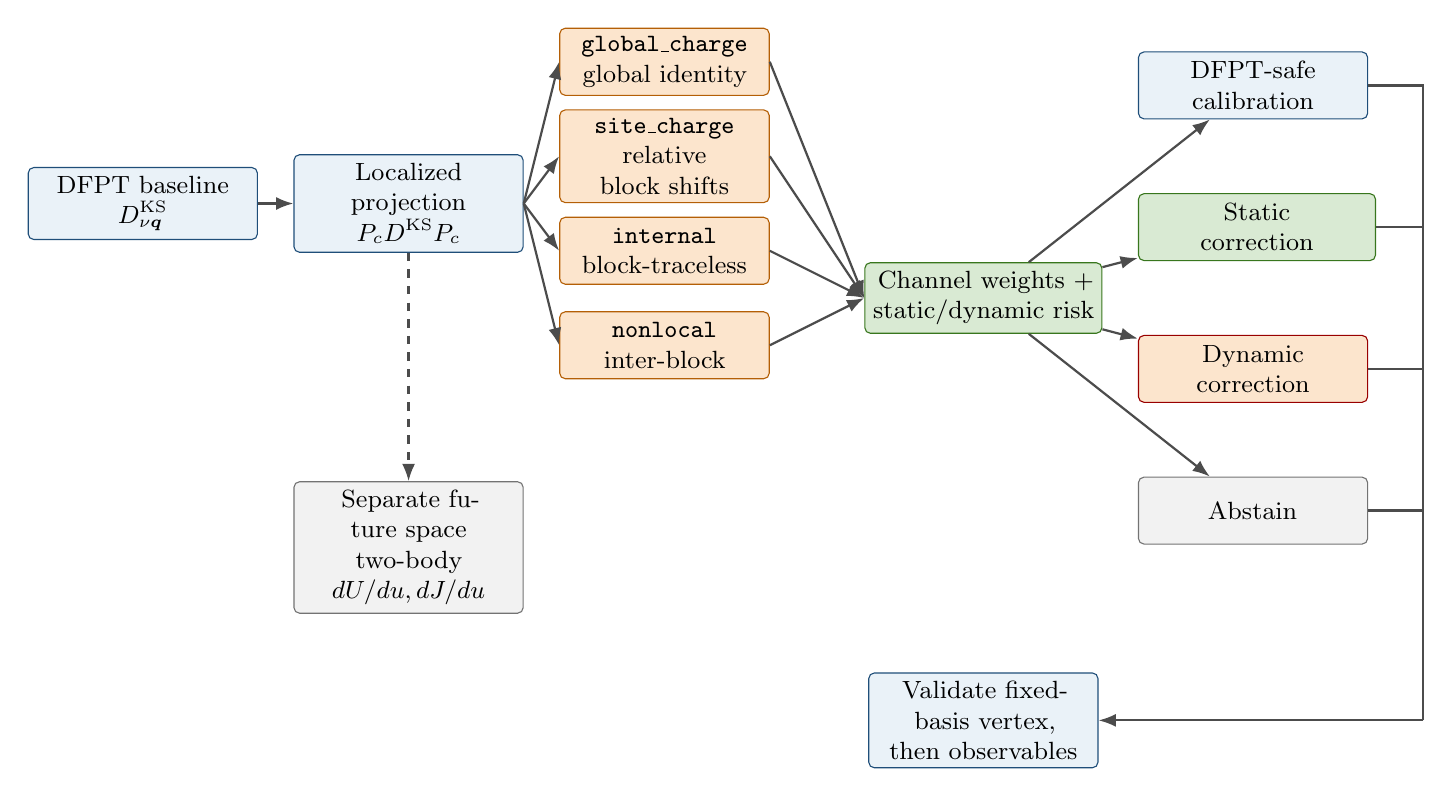
\begin{tikzpicture}[
  node distance=5.5mm and 4.5mm,
  box/.style={draw,rounded corners=2pt,align=center,font=\small,
              minimum height=8.5mm,text width=2.7cm,inner sep=3pt},
  base/.style={box,fill=softblue,draw=deepblue},
  channel/.style={box,fill=softorange,draw=deeporange,text width=2.45cm},
  decision/.style={box,fill=softgreen,draw=deepgreen,text width=2.8cm},
  arrow/.style={-{Latex[length=2.2mm]},thick,draw=black!70}
]
  \node[base] (dfpt) {DFPT baseline\\$D^{\ks}_{\nu\vq}$};
  \node[base,right=of dfpt] (project) {Localized projection\\$P_cD^{\ks}P_c$};

  \node[channel,right=of project,yshift=18mm] (global) {\texttt{global\_charge}\\global identity};
  \node[channel,right=of project,yshift=6mm] (site) {\texttt{site\_charge}\\relative block shifts};
  \node[channel,right=of project,yshift=-6mm] (internal) {\texttt{internal}\\block-traceless};
  \node[channel,right=of project,yshift=-18mm] (nonlocal) {\texttt{nonlocal}\\inter-block};
  \node[box,fill=black!5,draw=black!55,below=29mm of project]
    (twobody) {Separate future space\\two-body $dU/du,dJ/du$};

  \node[decision,right=12mm of internal,yshift=-6mm] (risk) {Channel weights +\\static/dynamic risk};

  \node[base,right=of risk,yshift=27mm] (safe) {DFPT-safe\\calibration};
  \node[decision,right=of risk,yshift=9mm] (static) {Static\\correction};
  \node[box,fill=softorange,draw=deepred,right=of risk,yshift=-9mm] (dynamic) {Dynamic\\correction};
  \node[box,fill=black!5,draw=black!55,right=of risk,yshift=-27mm] (abstain) {Abstain};

  \node[base,below=43mm of risk] (validate) {Validate fixed-basis vertex,\\then observables};
  \coordinate (merge) at ([xshift=6mm]static.east |- validate.east);

  \draw[arrow] (dfpt) -- (project);
  \foreach \x in {global,site,internal,nonlocal}
    \draw[arrow] (project.east) -- (\x.west);
  \foreach \x in {global,site,internal,nonlocal}
    \draw[arrow] (\x.east) -- (risk.west);
  \draw[arrow,dashed] (project.south) -- (twobody.north);
  \draw[arrow] (risk) -- (safe);
  \draw[arrow] (risk) -- (static);
  \draw[arrow] (risk) -- (dynamic);
  \draw[arrow] (risk) -- (abstain);
  \draw[thick,draw=black!70] (safe.east) -| (merge);
  \draw[thick,draw=black!70] (static.east) -| (merge);
  \draw[thick,draw=black!70] (dynamic.east) -| (merge);
  \draw[thick,draw=black!70] (abstain.east) -| (merge);
  \draw[arrow] (merge) -- (validate.east);
\end{tikzpicture}
}
  \caption{Proposed channel-resolved workflow.  DFPT supplies the baseline
  perturbation.  Projection and operator decomposition expose which physical
  channels a phonon drives.  A risk gate selects uncorrected DFPT, a static
  channel correction, or a dynamic calculation.  Validation is performed first
  on matrix elements and only then on observables.}
  \label{fig:framework}
\end{figure}

\subsection{Corrected perturbation and matrix element}

In a diagonal-channel approximation, define
\begin{equation}
  D^{\mathrm{next}}_{\nu\vq}(\omega)
  =D^{\ks}_{\nu\vq}
  +\sum_a\bigl[\mathcal K_a(\vq,\omega)-1\bigr]
   D^{(a)}_{\nu\vq}.
  \label{eq:dnext}
\end{equation}
The predicted quasiparticle coupling is
\begin{equation}
  g^{\mathrm{next}}_{mn\nu}(\vk,\vq,\omega)
  =\langle\psi_{m,\vk+\vq}|
    D^{\mathrm{next}}_{\nu\vq}(\omega)
    |\psi_{n,\vk}\rangle.
  \label{eq:gnext}
\end{equation}
When all $\mathcal K_a=1$, the method reduces exactly to its DFPT baseline.
Because the correction acts on operators before Bloch-state matrix elements are
taken, it preserves the band, momentum, and phase dependence already present in
DFPT.

\subsection{How each channel is corrected}

\paragraph{Charge channel.}
The implementation must enforce the exact uniform common-potential constraint and
pass a gauge/chemical-potential shift test.  At finite $q$, the UEG relation
\begin{equation}
  \mathcal K_{\rho}(q,0)
  \approx \frac{P(q,0)}{\chi_s(q,0)}
  \label{eq:uegprior}
\end{equation}
is a calibratable prior, not a universal crystal formula.  Crystal local-field
matrices, dimensionality, polar long-range fields, and multi-band screening must
be added explicitly.  A practical first model can fit the density kernel to a
small number of high-level $q$ points while imposing the exact $q=0$ anchor.

\paragraph{Local internal channels.}
For orbital splitting or mixing in a correlated subspace, obtain
$\partial_u\Sigma_{ab}(\omega)$ from finite-displacement DFT+DMFT, a linearized
impurity response, or a validated low-energy model.  If
$\eta_a^{\mathrm{dyn}}\ll1$, retain only $\mathcal K_a(\vq,0)$.  Near orbital,
spin-state, or Mott instabilities, the dynamic kernel and off-diagonal channel
mixing must be kept.

\paragraph{Nonlocal channels.}
When a phonon mainly changes hopping, hybridization, or long-range exchange, a
local impurity self-energy is insufficient.  Targeted GW perturbation theory,
finite-difference quasiparticle calculations, or a nonlocal embedding method can
provide selected matrix elements of $\mathcal K_{ab}$ \citep{Li2019}.  Symmetry
and locality can then interpolate those corrections over equivalent bonds and
wavevectors.

\paragraph{Interaction-modulation channels.}
If a displacement changes $U$, $J$, or another downfolded interaction, compute
those derivatives with constrained response and include the resulting two-body
vertex in the low-energy model.  Constrained DFPT provides a precedent for
separating screening processes during downfolding \citep{Nomura2015}.

\subsection{Three-level decision gate}

The framework chooses the least expensive level justified by diagnostics.

\begin{table}[htbp]
\centering
\caption{Decision levels for the proposed method.}
\label{tab:decisiongate}
\begin{tabularx}{\linewidth}{@{}p{2.6cm}XXp{3.2cm}@{}}
\toprule
Level & Physical diagnostic & Calculation & Required check \\
\midrule
DFPT-safe & Charge dominated; adequate reference bands; weak estimated dynamics
& Standard DFPT matrix elements & Gauge anchor and one representative high-level
control \\
Static correction & Internal or nonlocal weight is appreciable, but
$\eta^{\mathrm{dyn}}$ is small & Channel-projected static
$\mathcal K_a(\vq,0)$ & Held-out modes and momenta \\
Dynamic correction & Rapid vertex variation, soft electronic mode, small
coherence scale, or proximity to an instability & Frequency-dependent
$\mathcal K_{ab}(\vq,\omega)$ & Values across the physical phonon-frequency
window \\
Abstain & Outside the validated channel/basis/material domain & No automatic
prediction & Request a higher-level calculation \\
\bottomrule
\end{tabularx}
\end{table}

\subsection{Uncertainty and invariance requirements}

Every reported $g^{\mathrm{next}}$ should include uncertainty from high-level
training data, operator-basis choice, momentum interpolation, and neglected
channel mixing.  The following tests are mandatory:

\begin{itemize}
  \item invariance to unitary rotations within a declared degenerate orbital
  subspace;
  \item the acoustic sum rule and appropriate translational constraints;
  \item the uniform scalar-potential gauge test;
  \item Hermiticity and time-reversal/symmetry relations for
  $D^{\mathrm{next}}$; and
  \item recovery of uncorrected DFPT with $\mathcal K=I$.
\end{itemize}

\subsection{Why this is a new prediction framework}

Existing beyond-DFPT methods demonstrate how to compute particular corrections,
but they remain expensive when applied to all modes and wavevectors.  The proposed
novelty is the combination of (i) an operator-level physical diagnosis, (ii) a
hierarchical choice of correction theory, (iii) a low-dimensional transferable
kernel, and (iv) explicit uncertainty and abstention.  Its success criterion is
not that it matches a full many-body calculation by construction, but that it
predicts which parts of the DFPT matrix element need correction and reaches a
defined accuracy with far fewer high-level calculations.

\section{AI-agent research and implementation program}
\label{sec:program}

The AI agent is not used to replace physical validation.  Its role is to maintain
traceability across literature, material cases, calculations, code, and failed
hypotheses, while automating the repetitive parts of comparison and model
construction.

\subsection{Closed-loop workflow}

For each candidate material and phonon mode, the agent executes the following
auditable loop.

\begin{enumerate}
  \item \textbf{Read and extract.}  Search primary literature and record the
  material, mode eigenvector, $\vq$, electronic method, interaction parameters,
  definition and normalization of $g$, frequency at which the vertex is evaluated,
  and reported uncertainty.
  \item \textbf{Classify the perturbation.}  Project the DFPT perturbation,
  compute the charge, internal, and nonlocal channel weights of
  \cref{eq:channelstrength}, and attach a human-readable physical interpretation.
  \item \textbf{Select a benchmark.}  Choose the least expensive many-body method
  able to represent the active channel: UEG/vertex Monte Carlo for density,
  DFT+DMFT for local correlated channels, GW perturbation theory for nonlocal
  quasiparticle response, or an explicit model when interaction derivatives are
  central.
  \item \textbf{Generate a hypothesis.}  Propose a low-dimensional form of
  $\mathcal K_{ab}(\vq,\omega)$ with symmetry, Ward/gauge, locality, and causality
  constraints encoded before fitting.
  \item \textbf{Design a discriminating calculation.}  Select the mode or
  momentum point that maximizes disagreement between the current hypothesis and a
  plausible alternative, instead of merely adding more similar data.
  \item \textbf{Implement and test.}  Produce a versioned correction module,
  unit tests for algebraic invariants, and numerical regression tests against
  held-out high-level vertices.
  \item \textbf{Update or reject.}  Store negative evidence and revise the claim
  ledger.  The agent may not promote an empirical relation to an exact principle.
\end{enumerate}

Each extracted number must retain source, equation/table/figure location,
normalization convention, and whether it was read directly or inferred.  This is
essential because electron--phonon matrix elements can differ by phonon
normalization, spin factors, mode phase, orbital gauge, and screening convention.

\subsection{Minimal benchmark ladder}

The proposed ladder is designed to distinguish physical channels, not simply to
cover many chemical compositions.

\begin{table}[htbp]
\centering
\caption{Minimal benchmark ladder for developing and falsifying the method.}
\label{tab:benchmarks}
\begin{tabularx}{\linewidth}{@{}p{2.7cm}p{3.1cm}XX@{}}
\toprule
System & Active contrast & Reference level & Question answered \\
\midrule
Uniform electron gas & $q=0$ anchor versus $0<q\le2k_F$ density response &
Vertex diagrammatic Monte Carlo & Is the finite-$q$ density prior accurate and
what controls its residual? \\
SrVO$_3$ & Jahn--Teller versus breathing modes & DFT+DMFT & Does traceless orbital
weight predict the large mode-selective correction? \\
Doped CaCuO$_2$ & Half- versus full-breathing, static versus dynamic vertex &
DFT+DMFT & Can the dynamic-risk indicator detect failure of a static correction? \\
CoO & Correlated insulator and polar coupling & DFPT+$U$ / experiment & Does the
framework detect an invalid reference state and occupation-response channel? \\
Ba$_{1-x}$K$_x$BiO$_3$ or a simpler GWPT solid & Nonlocal quasiparticle response &
GW perturbation theory & Can a sparse nonlocal kernel reproduce the high-level
correction? \\
\bottomrule
\end{tabularx}
\end{table}

The UEG is the first diagnostic object because it isolates density physics.  It
must not be the only validation object, because success there cannot test internal
crystal channels.

\subsection{Accuracy, speed, and transparency metrics}

The target should be evaluated against three independent axes.

\paragraph{Accuracy.}
Report the error of complex matrix elements where phases are comparable, squared
couplings averaged on the relevant energy shell, and final observables.  A
practical initial threshold is to reduce the high-level-versus-DFPT error by at
least a factor of two while keeping the median corrected $|g|$ error below
10--15\% on held-out modes.  This threshold is a project criterion and may be
revised after the evidence matrix is complete.

\paragraph{Cost.}
Count the number of high-level displaced/response calculations, total core or GPU
hours, memory, and wall time relative to a dense many-body calculation of every
mode and $\vq$.  Speedup is meaningful only at comparable numerical convergence.

\paragraph{Transparency.}
For every prediction, output the operator decomposition, selected correction
level, training-source distance, uncertainty, and any violated invariant.  The
framework should expose why a mode was corrected rather than only returning a
number.

\subsection{Implementation layers}

The initial software can be separated into small testable modules:

\begin{enumerate}
  \item a reader for DFPT perturbation matrices and wavefunctions;
  \item localized-subspace construction and gauge checks;
  \item operator decomposition and Fermi-window channel weights;
  \item adapters for high-level reference data from UEG, DFT+DMFT, DFPT+$U$, and
  GWPT;
  \item constrained kernel fitting/interpolation with uncertainty;
  \item corrected-matrix-element reconstruction; and
  \item validation reports separating matrix-element and observable gates.
\end{enumerate}

No production implementation should begin before the two-day literature sprint
freezes the first hypothesis, the exact comparison quantities, and the first two
material-mode contrasts.

\section{Conclusions and immediate decision}
\label{sec:conclusions}

The apparent broad usefulness of DFPT should not be described as a mysterious
global cancellation.  DFPT computes a full, state-dependent static Kohn--Sham
response.  The missing many-body object is the phonon derivative of the
beyond-Kohn--Sham self-energy.  That derivative can be small for one perturbation
and large for another even when the equilibrium self-energy and mass enhancement
are large.

The clearest physical anchor is a uniform common potential coupled to conserved
total charge: it only changes the energy zero, so interactions cannot arbitrarily
renormalize it.  The Ward identity states this constraint precisely, but its
dynamic and static limits must not be confused.  The UEG extends the picture with
strong numerical evidence that a static density kernel remains accurate over
finite momenta up to $2k_F$ in the tested regime.  Because the UEG contains only
the density channel, this result suggests a compression principle rather than a
universal proof.

Real crystals add internal orbital, bond, hopping, hybridization, spin, and
interaction-modulation operators.  Existing DFT+DMFT, DFPT+$U$, and GWPT results
show that their corrections can be strongly mode-selective.  This motivates the
proposal's central hypothesis: the useful small parameter is not ``correlation
strength'' by itself, but the weight of a phonon in each operator channel times
the many-body amplification and dynamical variation of that channel.

The proposed next-generation calculation therefore retains DFPT, decomposes its
perturbation, and applies a channel kernel only where diagnostics demand it.  This
can be simpler and cheaper than computing a complete many-body vertex at every
mode and momentum while being more physically transparent than a black-box
correction to every matrix element.  It is not faster than the single DFPT
calculation used as its baseline.  Its current computational claim is narrower:
sparse higher-level anchors plus cheap inference can cost less than evaluating a
higher-level correction at every point.  A future speed claim against DFPT would
require a separately implemented surrogate for the DFPT coefficients and a
matched comparison with modern DFPT interpolation.

The accompanying software now fits a small channel-response matrix, predicts
held-out coefficient vectors, reports error, and compares DFPT-only, dense
higher-level, and sparsely corrected cost baselines.  It explicitly reports that
the present corrected path is not faster than DFPT.  Its bundled held-out vectors
are synthetic and its costs are normalized assumptions.  These results establish
reproducible software behavior, not material accuracy or a measured runtime
speedup.

\begin{keypoint}[First decision after submission]
The first research milestone should test one sharp statement: in SrVO$_3$, does a
basis-robust measure of traceless orbital-channel weight separate the strongly
enhanced Jahn--Teller mode from the weakly corrected breathing mode, while the UEG
density relation supplies the charge-channel control?  A positive result justifies
building the static prototype; a negative result forces the hypothesis to be
revised before software expansion.
\end{keypoint}


\appendix
\section{Detailed derivations and convention checks}
\label{app:derivations}

\subsection{DFPT response factorization in a scalar system}

Starting from \cref{eq:vksresponse,eq:chisresponse},
\begin{align}
  \delta V_{\ks}
  &=\delta V_{\mathrm{ion}}
   +(v+f_{\mathrm{xc}})\chi_s\delta V_{\ks},\\
  \bigl[1-(v+f_{\mathrm{xc}})\chi_s\bigr]\delta V_{\ks}
  &=\delta V_{\mathrm{ion}}.
\end{align}
With $P=\chi_s/(1-f_{\mathrm{xc}}\chi_s)$,
\begin{align}
  (1-vP)(1-f_{\mathrm{xc}}\chi_s)
  &=1-f_{\mathrm{xc}}\chi_s
   -v\frac{\chi_s}{1-f_{\mathrm{xc}}\chi_s}
       (1-f_{\mathrm{xc}}\chi_s)\\
  &=1-(v+f_{\mathrm{xc}})\chi_s.
\end{align}
Thus
\begin{equation}
  g^{\dfpt}
  =\frac{g^0}{(1-vP)(1-f_{\mathrm{xc}}\chi_s)}.
\end{equation}
Comparing with $g^{\mathrm{phys}}=g^0z\Gamma_\rho/(1-vP)$ yields
$z\Gamma_\rho=P/\chi_s$.  This algebra establishes the matching condition under
the scalar definitions; it does not establish that the condition is exact.

\subsection{Uniform-potential cancellation at a quasiparticle pole}

Let the pole satisfy
\begin{equation}
  E_u-\varepsilon-Du-\Sigma_0(E_u-Du)=0.
\end{equation}
Differentiate at $u=0$:
\begin{equation}
  \frac{dE}{du}-D
  -\partial_\omega\Sigma_0\left(\frac{dE}{du}-D\right)=0.
\end{equation}
Provided the pole is well-defined,
$(1-\partial_\omega\Sigma_0)(dE/du-D)=0$, so $dE/du=D$.  In the alternative
form where $\partial_u\Sigma=-D\partial_\omega\Sigma$, the same result is
$z(D+\partial_u\Sigma)=D$ with
$z=(1-\partial_\omega\Sigma)^{-1}$.  The result follows from the common shift of
frequency and chemical potential, not from weak interaction.

\subsection{Limit ordering in the Ward identity}

Expand the right-hand side of \cref{eq:ward} for small four-momentum:
\begin{equation}
  G^{-1}(k+q)-G^{-1}(k)
  =\ii\nu\,\partial_{\ii\omega}G^{-1}
   +\vq\cdot\nabla_{\vk}G^{-1}+\order(q^2).
\end{equation}
At $\vq=0$, matching the coefficient of $\ii\nu$ gives the scalar dynamic
vertex.  At $\nu=0$, matching the coefficient of $\vq$ gives the longitudinal
current vertex.  A static scalar perturbation also changes the distribution and
self-consistent field, producing the compressibility vertex.  This explicit
expansion shows why swapping the two limits changes the conclusion.

\subsection{Matrix generalization}

In a crystal, $v$, $P$, $\chi_s$, $f_{\mathrm{xc}}$, and $\epsilon$ are matrices
in reciprocal vectors $\bm G,\bm G'$.  Products do not generally commute, so the
scalar factorization in \cref{eq:factorization} cannot be transferred by simply
replacing every scalar with a matrix.  A crystal implementation must retain
matrix ordering and local-field components, or derive a controlled projected
version of the relation.  This is one of the first theoretical tasks of the
project.

\section{Evidence matrix}
\label{app:evidence}

\small
\begin{longtable}{@{}p{2.4cm}p{2.55cm}p{2.25cm}p{2.45cm}p{3.2cm}@{}}
\caption{Current evidence for and against the working hypothesis.  Numerical
values follow the normalization reported in the cited studies and must be checked
again before cross-code fitting.}
\label{tab:evidence}\\
\toprule
System / mode & DFPT or baseline & Higher-level result & Dominant interpretation &
Status and use \\
\midrule
\endfirsthead
\toprule
System / mode & DFPT or baseline & Higher-level result & Dominant interpretation &
Status and use \\
\midrule
\endhead
\bottomrule
\endfoot
Strict uniform common potential & Bare/common shift $D$ & Exact pole shift $D$ &
Conserved total charge / energy-zero shift & Exact anchor; no finite-$q$
scattering claim \\

UEG, $0\le q\le2k_F$, $r_s=1$--$5$ & Static DFPT-like density kernel &
Vertex diagrammatic Monte Carlo & Single scalar density channel & Recent preprint
evidence for finite-$q$ compression; not a theorem \citep{Cai2025} \\

SrVO$_3$, M-point Jahn--Teller & about $44$ meV & about $87$ meV at $\omega=0$ &
Traceless orbital splitting & Strong positive example for an unprotected internal
channel \citep{Abramovitch2025} \\

SrVO$_3$, R-point breathing & about $58$ meV & about $50$ meV at $\omega=0$ &
More charge-like local modulation & Same-material control; modest static correction
\citep{Abramovitch2025} \\

Doped CaCuO$_2$, half breathing & about $70$ meV & about $76$ meV at $\omega=0$ &
Charge-transfer / bond response & Modest static correction at representative $U$
\citep{Abramovitch2025} \\

Doped CaCuO$_2$, full breathing & about $53$ meV & about $45$ meV at $\omega=0$ &
Charge-transfer / bond response & Modest negative static correction at
representative $U$ \citep{Abramovitch2025} \\

Doped CaCuO$_2$, larger $U$ & Static value may appear moderate & Strong
$\omega$ dependence on phonon scale & Low coherence scale / dynamic local vertex &
Counterexample to using only a static correction \citep{Abramovitch2025} \\

CoO, polar coupling & Semilocal DFPT reference is qualitatively deficient &
DFPT+$U$ changes electronic structure and Fr\"ohlich coupling & Correlated
occupation response plus polar screening & Established standard-DFPT limitation
\citep{Zhou2021} \\

Ba$_{1-x}$K$_x$BiO$_3$ & DFT linear response & GW perturbation theory enhances
coupling & Nonlocal and energy-dependent quasiparticle response & Established
beyond-DFT derivative route \citep{Li2019} \\
\end{longtable}
\normalsize

The matrix is deliberately organized by perturbation type rather than by a single
material-wide correlation label.  Its central unresolved test is whether the
operator decomposition predicts the observed contrast without fitting each mode
independently.

\section{Two-day literature and hypothesis-freeze protocol}
\label{app:twoday}

The initial exploration is limited to two days.  Its purpose is not to survey the
entire electron--phonon literature, but to decide whether the channel-selective
hypothesis is physically defensible and to freeze the first decisive comparison.

\subsection*{Day 1: establish constraints and collect contrasts}

\begin{enumerate}
  \item \textbf{Morning: foundations.}  Verify the DFPT response convention,
  physical quasiparticle vertex, proper versus screened vertex, Ward identity, and
  static/dynamic limit ordering from primary sources
  \citep{Baroni2001,Giustino2017,Hedin1965,Nambu1960}.
  \item \textbf{Midday: UEG.}  Reproduce the algebra of
  \cref{eq:matchingcondition,eq:propervertexmatching}; verify that the complete
  $K_{\mathrm{total}}\simeq1$ rather than applying the proper-vertex ratio twice;
  extract the reported $q$, $r_s$, temperature, and
  error ranges from \citet{Cai2025}; list which statements are numerical and which
  are exact.
  \item \textbf{Afternoon: correlated contrasts.}  Extract mode definitions,
  eigenvectors, parameters, normalization, static vertices, and frequency
  dependence for SrVO$_3$ and CaCuO$_2$.

  The primary source is \citet{Abramovitch2025}.  Add CoO and one GWPT case to
  identify failure mechanisms not represented by local DMFT.
  \item \textbf{Evening gate.}  Produce a one-page evidence table with at least
  one supporting and one challenging case for each proposed channel.
\end{enumerate}

\subsection*{Day 2: turn the idea into a falsifiable first experiment}

\begin{enumerate}
  \item \textbf{Morning: define observables.}  Freeze the localized subspace,
  operator normalization, Fermi-window weights, target $g$ convention, and basis
  robustness checks.
  \item \textbf{Midday: compare alternatives.}  Test at least three hypotheses on
  the evidence table: correlation strength alone, quasiparticle residue alone,
  and channel weight times channel susceptibility.  Record which observations
  each cannot explain.
  \item \textbf{Afternoon: design the first calculation.}  Select a SrVO$_3$
  Jahn--Teller/breathing contrast and a UEG density control.  Represent the
  finite-R mode in the phase-correct $2\times2\times2$ real supercell or equivalent
  standing-wave basis before assigning channel weights.  Specify input data, code
  path, acceptance thresholds, and the result that would reject the channel hypothesis.
  \item \textbf{Final gate.}  Freeze one paragraph stating the physical
  hypothesis, one equation for the first correction model, one benchmark table,
  and one stop/go decision for implementation.
\end{enumerate}

\subsection*{Required outputs after 48 hours}

\begin{itemize}
  \item a source-checked evidence matrix with no mixed normalization conventions;
  \item a claim ledger labeling exact results, established methods, numerical
  evidence, and hypotheses;
  \item the first two material/mode comparisons and their input availability;
  \item a minimal operator-decomposition prototype specification; and
  \item an explicit decision: implement, revise the hypothesis, or stop.
\end{itemize}

The literature sprint is successful only if it reduces uncertainty about the
physical hypothesis.  The number of papers read is not itself a success metric.

\section{Claim ledger: what is known and what is proposed}
\label{app:claims}

\begin{longtable}{@{}p{2.4cm}p{8.2cm}p{3.1cm}@{}}
\caption{Epistemic status of the central statements.}
\label{tab:claims}\\
\toprule
Status & Statement & Main support \\
\midrule
\endfirsthead
\toprule
Status & Statement & Main support \\
\midrule
\endhead
\bottomrule
\endfoot
\claimstatus{Established} & Standard adiabatic DFPT is a self-consistent static
Kohn--Sham response and computes the matrix element of
$\partial_{\nu\vq}V_{\ks}$. & \citet{Gonze1995,Baroni2001,Giustino2017} \\

\claimstatus{Established} & The many-body response closes screening,
polarization, self-energy, and a vertex; they are not three arbitrary independent
factors. & \citet{Hedin1965} \\

\claimstatus{Exact limit} & A strict uniform common scalar potential coupled to
total charge is an energy-zero shift; the corresponding dynamic Ward limit gives
$z\Gamma^0_\omega=1$. & \citet{Nambu1960} and
\cref{app:derivations} \\

\claimstatus{Limitation} & The static $\vq\to0$ density response is not fixed by
$z\Gamma=1$ alone; finite-$q$ density is not a conserved operator. & Ward limit
ordering and Fermi-liquid compressibility \\

\claimstatus{Numerical evidence} & In the tested UEG regime, a DFPT-like static
density-kernel vertex agrees accurately with a high-level vertex over momenta up
to $2k_F$. & \citet{Cai2025}; recent preprint \\

\claimstatus{Numerical evidence} & Beyond-DFPT corrections can differ strongly
between phonons in the same correlated material and can be frequency dependent. &
\citet{Abramovitch2025} \\

\claimstatus{Working hypothesis} & Channel content times channel-resolved
many-body amplification is a better predictor of DFPT error than $U$ or $z$
alone. & Proposed here; to be tested on \cref{tab:benchmarks} \\

\claimstatus{Proposed method} & A small static/dynamic operator kernel can correct
DFPT with substantially fewer high-level calculations than a full vertex grid. &
\cref{sec:nextdfpt}; not yet validated \\

\claimstatus{Open question} & The scalar UEG matching condition has a useful,
basis-robust matrix generalization in a crystal with local fields and multiple
orbitals. & First formal task after the literature sprint \\
\end{longtable}


\bibliographystyle{unsrtnat}
\bibliography{references}

\end{document}
